\documentclass[letterpaper]{article}
\usepackage[utf8]{inputenc}

\usepackage{ifxetex}
\ifxetex
  \usepackage{fontspec}
  \setmainfont[ExternalLocation=../Common/, 
              		  Ligatures =TeX,
					  BoldFont = Cabin-Bold.ttf,
					  ItalicFont = Cabin-Italic.ttf,
					  BoldItalicFont = Cabin-BoldItalic.ttf ]
					  {Cabin-Regular.ttf}
\fi

\title{\huge DK2 Specification}
\author{Nirav Patel\\ Nate Mitchell\\ Kam Chin\\ Ryan Brown}
\date{Revision 0.4\\
30 May 2014}

\usepackage{parskip}
\usepackage{graphicx}
\usepackage{hyperref}
\usepackage{color}
\usepackage{fancybox}
\usepackage[usenames,dvipsnames,svgnames,table]{xcolor}
\usepackage{fancyhdr}
\usepackage{todo}
\usepackage{mdwlist}
\usepackage{float}
\pagestyle{fancy}
\definecolor{lightgray}{gray}{0.8}
\renewcommand{\arraystretch}{1.25}

\begin{document}

\begin{figure}

\includegraphics[width=5in]{Figures/OculusLogo.png}
\end{figure}

\maketitle
\thispagestyle{empty}

\lfoot{DK2 Specification 0.4}
\cfoot{}
\rfoot{\thepage}

\newpage

\tableofcontents

\newpage

\section{Revision History}

\begin{center}
    \begin{tabular}{ | l | l | p{8cm} |}
    \hline
    \cellcolor{lightgray} Revision & \cellcolor{lightgray} Date & \cellcolor{lightgray} Description \\ \hline
    0.1 & 18-9-2013 & Preliminary specification. \\ \hline
    0.2 & 3-10-2013 & Modifications from specification review. \\ \hline
    0.3 & 5-22-2014 & Updated to current design. \\ \hline
    0.4 & 5-30-2014 & Updates to cable and optics. \\ \hline
    \end{tabular}
\end{center}

\newpage

\section{Introduction}
The Oculus Rift is a virtual reality headset designed for immersive gaming. Development Kit 2 (DK2) is the second iteration of the development kit that game developers use to build games and applications for the consumer version of the Rift. \\

DK2 introduces a number of new features over DK1, including:

\begin{itemize}
    \item Higher image quality via a 1080x1920 pixel resolution AMOLED display
    \item Positional head tracking via an external Positional Tracker and headset IR LEDs    
    \item Extensibility via a user accessible USB port
\end{itemize}

\newpage

\section{Box Contents}
The Oculus Rift Development Kit 2 includes the following:

\begin{itemize}
    \item Headset with detachable cable
    \item Lenses - 2 sizes and cleaning cloth
    \item Positional Tracker
    \item Positional Tracker USB cable
    \item Positional Tracker sync cable
    \item 1 DVI to HDMI adapter
    \item Power adapter and 4 plugs: US (attached), UK, AU, EU
\end{itemize}

\newpage

\section{Primary Vendors}

\begin{itemize}
    \item Vishay
    \item STMicroelectronics
    \item Toshiba
    \item Richtek
    \item InvenSense
    \item Samsung Display
    \item Berway
    \item Jabil
    \item Elka
    \item Cypress
    \item Coxon
    \item Aptina
    \item Etron
    \item Boowon
\end{itemize}

\newpage

\section{Industrial and Mechanical Design}
DK2 is designed to be comfortable, lightweight, and durable for Virtual Reality game and content developers.  The industrial design is comprised of three distinct sections: the physical plastic panel, optics, and electronics housing, the foam and rubber facial interface, and mounting straps.  The total weight of the unit is 440 grams.

\subsection{Housing}
The DK2 headset shell is outer front cover and designed for IR transmissive cover for position tracking LEDs. This shell shape is unique industrial design and consists cable door, power button, power light pipe, Aux/USB light pipe and rubber plug. It also cover for HMD controller board. The shell interconnects with DK2 cable and Facial Interface. It has a dedicated location for product label behind both connectors. The shell has a nose recess allowing for nose clearance when the shell is assembled to other optical mounting base.

\begin{center}
    \begin{tabular}{ | l | p{8cm} |}
    \hline
    \cellcolor{lightgray} Parameter & \cellcolor{lightgray} Specification \\ \hline
    Housing & Black plastic injection molded ABS IR Transmissive \\ \hline
    Weight & 97.5 grams \\ \hline
    Finish & Matte (Sandblasted Tool) \\ \hline
    \end{tabular}
\end{center}

\begin{figure}[H]  
  \centering
    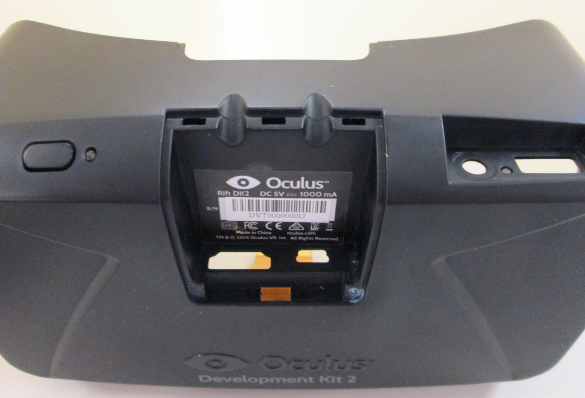
\includegraphics[width=0.92\textwidth]{Figures/image2-17.png}
\end{figure}

\subsection{Internal Structure}
The DK2 Mounting Base is inner part of the HMD unit where optics and panel are mounted together. Two eyecups are mounted into the Mounting Base from user viewing side and panel with rubber cushion is mounted on the other side of the Base with Frame. 
The mounting base design is highly leveraged from DK1. The Base is an interface part for Front Cover Shell and Facial Interface. The Base has a nose recess and maximized for nose clearance and optical viewing.

\begin{center}
    \begin{tabular}{ | l | p{8cm} |}
    \hline
    \cellcolor{lightgray} Parameter & \cellcolor{lightgray} Specification \\ \hline
    Housing & Black plastic injection molded ABS \\ \hline
    Weight & 176.5 grams \\ \hline
    Finish & Matte (light textured tool) \\ \hline
    \end{tabular}
\end{center}

\begin{figure}[H]  
  \centering
    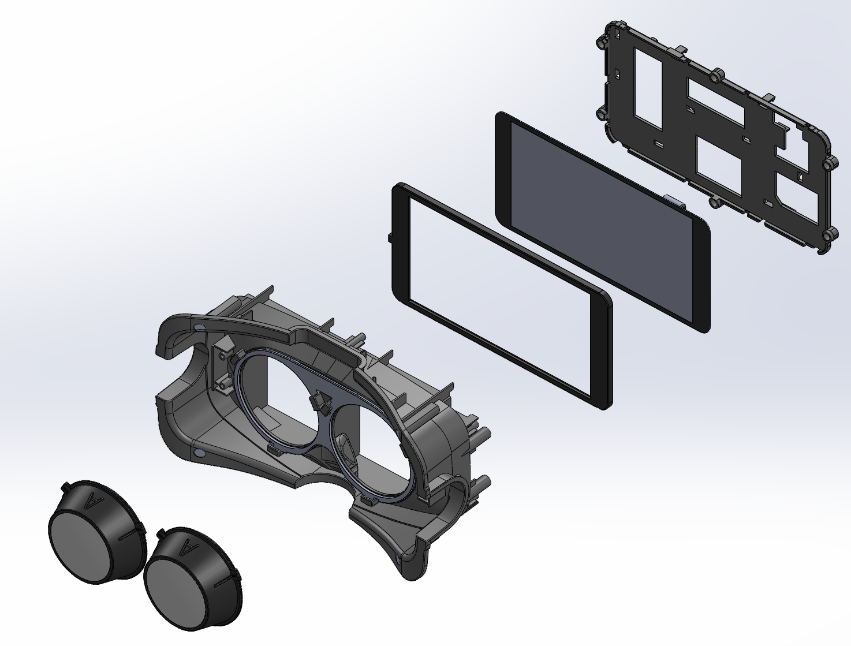
\includegraphics[width=0.92\textwidth]{Figures/image8-29.png}
\end{figure}

\subsection{Eye Relief Adjustment}

To allow for a wide variety of face shapes, the entire housing assembly containing the panel and optics can be adjusted closer and farther from the user's face using a coin on the mechanisms on the left and right sides of the headset.

\subsection{Facial Interface and Straps}
The facial interface of DK2 attaches to the housing using a multi-clip system. The primary components are a curved rubber mask, mesh ventilation openings, and a strip of microfiber covered triple-layer die cut foam attached to the mask with a layer of adhesive. The facial interface is very similar in design to that of ski goggles, with many of the same objectives: long term comfort, sweat resistance, and durability. \\

The DK2 Straps and Facial Interface design are carried over from DK1. Top strap design is highly leverage from DK1 and with two additional elastic cable loops. One loop is located in the front of the strap and 6 to 9 mm away from hard plastic loop. And, another loop is located in the back of the strap where T-shaped clip located and in vertical orientation. The Loop is able to stretch for connector insertion and holding cable in place. Right side of the adjustable strap loop is the same as left side loop unlike DK1 right side loop with cable clip feature.
Facial Interface?s plastic part bridge portion is trimmed off where nose clearance is located from DK1 design.

\begin{center}
    \begin{tabular}{ | l | p{8cm} |}
    \hline
    \cellcolor{lightgray} Parameter & \cellcolor{lightgray} Specification \\ \hline
    Weight & 138 grams \\ \hline
    Facial interface & Single layer die-cut foam strip, flexible PPU mounting \\ \hline
    Facial interface foam dimensions & Approximate 14mm thick, 19mm wide \\ \hline
    Straps & Two nylon/elastic fabric straps attached to the left and right sides of the headset. Top Strap has Velcro for ease of adjustment \\ \hline
    Strap Dimensions & Top strap: 3.5 mm thick, 30 mm wide, 420 mm length (approximate).
Side strap: 2.6 mm thick, 39.5 mm wide, 220 mm length (approximate) \\ \hline
    \end{tabular}
\end{center}

\begin{figure}[H]  
  \centering
    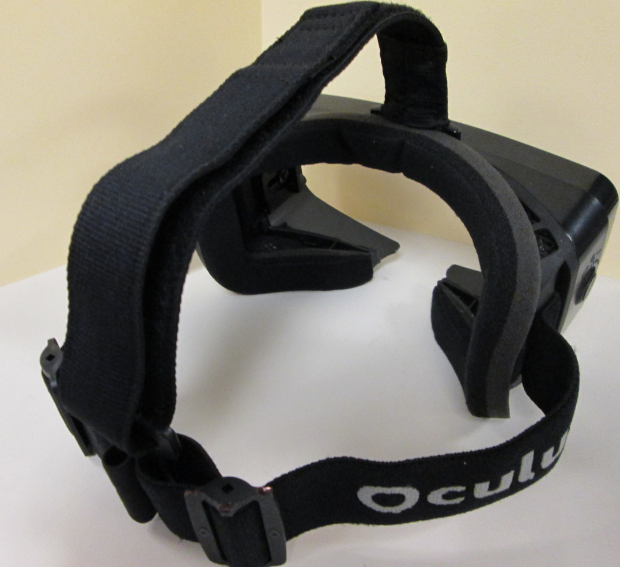
\includegraphics[width=0.92\textwidth]{Figures/image4-21.png}
\end{figure}

\subsection{Tracking LEDs}
DK2 includes 40 Vishay VSMY3850 850nm IR LEDs for positional tracking. These LEDs are reflow soldered onto an FPC which is attached to the inside of the front plate of the headset using 3M VHB double sided tape. They are spaced approximately 30mm apart in a design defined by computer vision algorithms.

\newpage

\subsection{Interface Control}
The Rift has a momentary tactile switch used for powering on and off.

\subsection{Status Indicator}
A bi-color amber/blue status LED on the Rift shows indication of power on as well as notification of errors.  The LED is located next to the power button.  Amber indicates that the headset is powered but not receiving video input.  Blue indicates that the headset is powered and receiving video input.

\subsection{USB Port}
A user accessible USB port is available on the top surface of the Rift.  A 2.5mm synchronization jack is placed next to the USB port to allow for synchronization of the .  The USB port is enabled and providing up to 500 mA only when the optional wall wart power is plugged in to the DK2 Cable.

\newpage

\section{Optics}
The design of the viewing optics is to cover human visual field based on biological and psychological researches. Having a single lens approach for cost effectiveness, the design is optimized not only in optics but also in image processing. There are two sets of magnifiers, labeled A and B, for the user's eye sight or preference. Each magnifier is placed at 10mm in front of each eye, situated with their centers 63.5mm (as an average inter-pupillary distance) apart. The A eyecup is mounted for normal 20/20 eye vision and B eyecup is for near-sighted users.

\begin{center}
    \begin{tabular}{ | l | p{8cm} |}
    \hline
    \cellcolor{lightgray} Parameter & \cellcolor{lightgray} Specification \\ \hline
    Lens Material & Molded optical-grade polycarbonate \\ \hline
    Lens Thickness & 5.36mm thick at the edge and 15mm at the center. \\ \hline
    Lens Type & Aspherical \\ \hline
    \end{tabular}
\end{center}

\begin{figure}[H]  
  \centering
    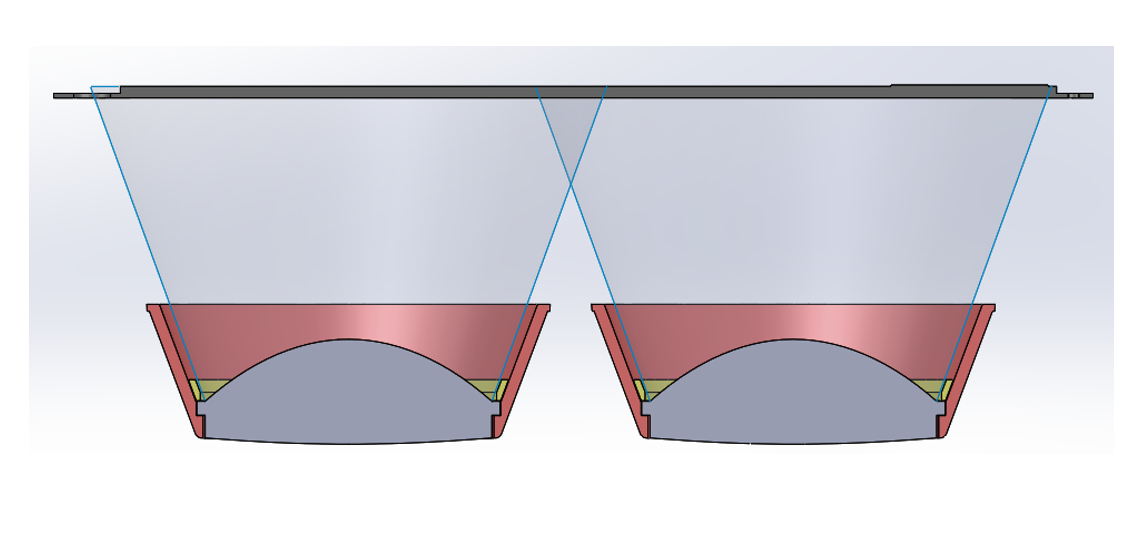
\includegraphics[width=0.92\textwidth]{Figures/image1-15.png}
\end{figure}

\begin{figure}[H]  
  \centering
    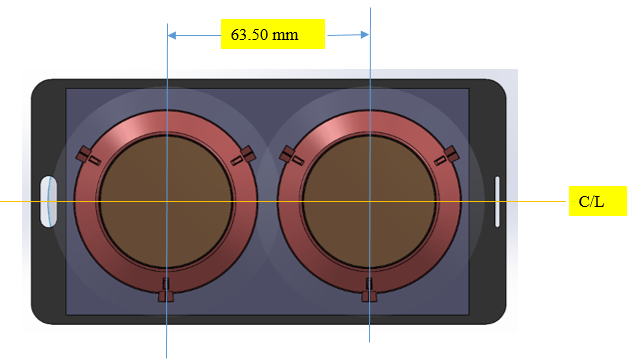
\includegraphics[width=0.92\textwidth]{Figures/image7-27.png}
\end{figure}

\subsection{Focus Adjustment}
To accommodate near-sighted users, an additional pair of lens cups labelled B are included with the DK2 with a 2.5mm shorter focal length.  The default lens cups installed in the headset are labelled A.  \\ 

\newpage

\section{Display}
DK2 uses a 5.68" Full HD AMOLED panel developed by Samsung Display. It is a portrait mode driven display viewed in landscape orientation, with each eye viewing half of the active screen area for a per-eye resolution of 960x1080.

\subsection{Panel}
The Samsung Display AMS568 is an RGBG pentile AMOLED panel measuring 5.68" diagonally with a 16:9 aspect ratio and a total resolution of 1080x1920. The viewable area dimensions are 70.74mm x 125.76mm.  The panel stackup from bottom to top is a foam layer, the LTPS layer, encapsulation, a polarizer, optical adhesive, a touch screen, and cover glass.  The touch screen layer is not powered or interfaced in the DK2 headset.  The module weight is 36.4 grams.

\subsection{Display Driver}
The display driver on the panel is the Samsung S6E3FA0, which supports 4 lane MIPI-DSI at up to 1.1 Gbps per lane.

\subsection{Brightness Control}
Analog voltage rails for the panel are supplied by a the TI TPS65633 triple output power supply.  The ELVSS rail can be controlled by the panel to adjust brightness.  Brightness control is made available via the Oculus SDK.  A HID Control report sets the the desired level to the microcontroller on the Rift, which then writes the request via i\textsuperscript{2}c to the display controller, which sends the MIPI DCS command to the panel to adjust the ELVSS level.  The default brightness of the headset is approximately 100 nit.

\subsection{Low Persistence Mode}
Although the effectively instant pixel switch times on an AMOLED reduce motion blur relative to LCDs, a perceptual artifact results in a specific type of motion blur called judder remaining.  Michael Abrash's blog posts offer thorough explanations of the perception of and challenges around judder.

\begin{itemize}
  \item \url{http://blogs.valvesoftware.com/abrash/why-virtual-isnt-real-to-your-brain-judder/}
  \item \url{http://blogs.valvesoftware.com/abrash/down-the-vr-rabbit-hole-fixing-judder/}
\end{itemize}

The summary is that during smooth pursuit by the eye of an object moving across space or during the vestibulo-ocular reflex (VOR) in which the eye tracks a stationary object in space smoothly as the head rotates, the object appearing on the display remains stationary for a full frame length of 16.6ms while the eye continues to rotate to track the expected path of its motion.  The effect is that the object perceptually is smearing across the retina as the eye continues to turn while the image remains stationary.  This can be most easily observed by attempting to read text fixed in the virtual environment as the head turns.  The text appears blurry as the eye attempts to track it.

The significance of the effect is proportional to the angular velocity of the head or moving object and the length of time that the object persists on the display.  The solution to the problem is therefore to reduce the length of time that the object persists on the display.

DK2 accomplishes this using a feature of the AMS568 panel called AID, which allows for rows to be enabled in a rolling manner on a reduced duty cycle.  The default duty cycle for the DK2 headset is 22.5\%.  The duty cycle is adjustable through a HID report write using the Oculus SDK.

\newpage

\section{Positional Tracker}
The Positional Tracker uses an Aptina MT9V034 sensor and an Etron eSP570 USB controller.  A user removable band pass filter on the outside of the lens stack allows for high efficiency infrared tracking as well as visible light use.  The Positional Tracker is interfaced to the host PC via a USB Mini jack as well as to the DK2 Cable via a 2.5mm synchronization jack.  See the DK2 Positional Tracker Specification for details on the positional tracking system.

\newpage

\section{Mainboard}
The mainboard of DK2 contains the video interface circuitry, the Tracker, the LED driving circuitry, and a USB hub.  See the DK2 Mainboard Specification for implementation.

\begin{figure}[H]  
  \centering
    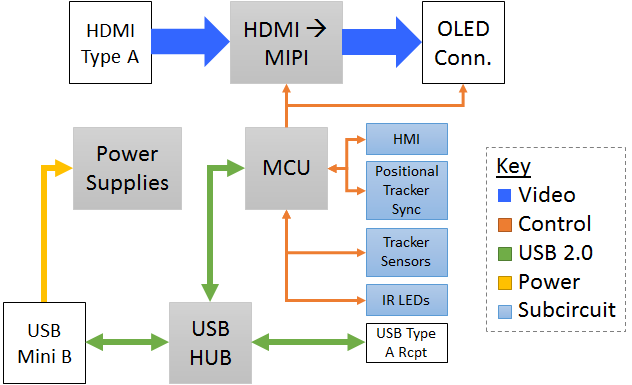
\includegraphics[width=0.92\textwidth]{Figures/DK2_Mainboard.png}
  \caption{Rift DK 2 Mainboard Diagram}
  \label{Mainboard_Diagram}
\end{figure}

The mainboard uses a 6 layer FR4 PCB to accommodate high speed impedance matched differential pairs.

\subsection{Power}
The DK2 power system generates all required voltages from the 5V input, optimized for minimal coversion loss.  The following rails are used:

\begin{itemize}
    \item 3.3V, 1.2V from a buck regulator
    \item 3.0V from an LDO from 3.3V
    \item 2.0V from a buck regulator
    \item 4.6V, 7.0V, -4.4V from a TPS65633
\end{itemize}

The total power consumption is under 500 mA to allow the product to be bus powered.

\subsection{HDMI MIPI Bridge}
To interface the HDMI input signal to the MIPI-DSI panel, a Toshiba TC358779 HDMI MIPI Bridge is used.  The TC358799 is a 64 ball BGA package.  It takes HDMI input at an up to 165 MHz pixel clock, optionally upscales and color adjusts it, and outputs it over a four lane MIPI-DSI interface.  The device is configured by the microcontroller over i\textsuperscript{2}c.\\

The TC358799 natively supports HDCP.  DK2 uses HDCP keys provided by Toshiba.

\begin{center}
\fcolorbox{black}{lightgray}{\parbox{\textwidth}{\textbf{Note}\\The TC358799 does not support video rotation or superposition of an on-screen display (OSD).}}
\end{center}

\subsubsection{EDID}
The HDMI DDC lines interface to a dedicated EDID EEPROM.  The EEPROM is programmed at the factory and can also be updated via the microcontroller.  The EDID contains the following display modes:

\begin{itemize*}
    \item 1080x1920 75 Hz (default)
    \item 1080x1920 60 Hz
    \item 1080x1920 72 Hz 
\end{itemize*}

The Product ID in the EDID is 0x04.  The display serial number presented in the EDID matches that of the microcontroller on the USB interface.

\subsection{USB Hub}
The mainboard contains a Cypress CY7C65634-28LTXC \footnote{\url{http://www.cypress.com/?mpn=CY7C65634-28LTXC}} 2-port USB hub.  One port interfaces to the Tracker microcontroller, while the other is connected to a USB Type A port exposed on the headset for use by the user.\\

A USB overcurrent detection and control IC interfaced to the hub powers the user USB port to ensure that overcurrent devices are disconnected.\\

When DK2 is bus powered, the user USB port is disabled.  With DK2 self powered by a wall wart, the port advertises 500 mA capability.  The hub is configured using the microcontroller to set and change this information.

\newpage

\section{Microcontroller and Sensors}
The DK2 microcontroller is a USB 2.0 FS HID device which reports inertial sensor information to the host PC, as well as allowing for driver free control of various Rift functions.  The microcontroller system is a component of the Mainboard.

\subsection{Microcontroller}
An STMicroelectronics STM32L100R8T6\footnote{\url{http://www.st.com/web/catalog/mmc/FM141/SC1169/SS1295/LN1808/PF255678}} Cortex-M3 microcontroller handles the USB interface, interfacing to the various sensors on the main board, configuring the HDMI MIPI bridge, and configuring the tracking LEDs.  Dual-stage firmware allows for the application firmware to be updated by a bootloader over USB HID.

\subsection{Gyroscope and Accelerometer}
An Invensense MPU-6500\footnote{\url{http://www.invensense.com/mems/gyro/mpu6500.html}} 3-axis gyroscope and accelerometer handles reporting angular velocity and acceleration information to the PC, allowing for low latency orientation measurement.  The sensor supports a 1000 Hz sampling rate, and reports 16-bit per axis data over SPI.

\subsection{Magnetometer}
An STMicroelectronics LIS3MDL\footnote{\url{http://www.st.com/web/en/catalog/sense_power/FM89/SC1449/PF255198}} 3-axis magnetometer reports magnetic field data back to the PC, allowing for yaw correction of the orientation data.  The device reports over SPI with 16-bit data for all axes at a 80 Hz update rate.

\subsection{Sampling Synchronization}
Sensor samples also contain a bit indicating the display VSYNC pulse, allowing the tracking LEDs and tracking frames to be time synchronized with inertial measurements.

\subsection{Latency Tester}
The microcontroller reads the top left pixel off of the display controller each frame, sending it back to the PC in the sensor HID reports.  This allows precise continuous latency measurements to the developer and to the sensor fusion prediction algorithm.

\newpage

\section{Firmware}
The STM32L100 microcontroller on the mainboard with 128 KB of Flash contains two stages of firmware, the Bootloader and the Application.

\subsection{Bootloader}
The Bootloader firmware runs immediately on powering the headset.  If no firmware update flag was set, the Bootloader jumps to the Application firmware.  If a firmware update flag was set through previous running of the Application firmware or by holding the power button when powering on, the Bootloader firmware jumps to a mode where it is able to receive new Application firmware over the USB interface.  This allows for field updates of Application firmware.  See the Oculus Bootloader Specification for further details.

\subsection{Application}
The Application firmware interfaces to the host PC over USB to transmit sensor and timestamp data at up to 1000 Hz as well as receive configuration commands for the sensors, tracking LEDs, and display.  Calibration parameters for the LEDs, sensors, and lenses are also stored in EEPROM accessed by the Application firmware.  See the DK2 Firmware Specification for further details.

\newpage

\section{Cable}
The USB, power, and video cable for DK2 is detachable.  This custom cable allows for USB, HDMI, and power to be contained within a single 3 meter cable assembly for minimal diameter and maximum flexibility.  The HMD (sink) side of the cable connects to a HDMI Type A and a USB Mini B inline on the top of the headset.  The sink side HDMI connector contains a Spectra7 VR7100 HDMI equalizer.

On the PC (source) side, the cable breaks out into two 1 foot tails, one for HDMI Type A and one for USB Type A.  The breakout also contains a barrel connector for optional 5V power input and a 2.5mm connector for the sync signal to the Positional Tracker.  Full details on the cable are available in the DK2 Cable Specification.

\newpage

\begin{figure}[H]  
  \centering
    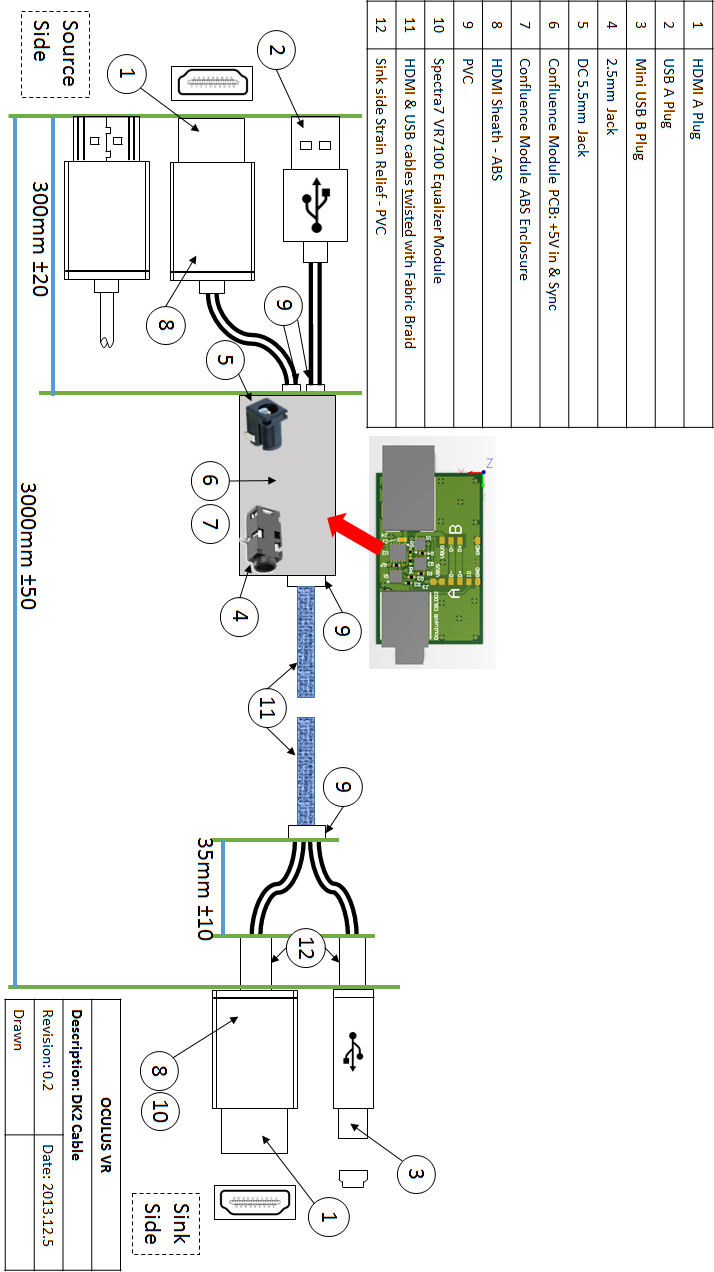
\includegraphics[width=0.88\textwidth]{Figures/DK2_Cable_Drawing.png}
  \caption{Rift DK 2 Cable Drawing}
  \label{Cable_Diagram}
\end{figure}

\newpage

\subsection{Molded Components}
The DK2 Cable includes custom molded backshells, confluence module enclosure, and strain relief - detailed in the following table.

\begin{center}
    \begin{tabular}{ | l | l | p{8cm} |}
    \hline
    \cellcolor{lightgray} Parameter & \cellcolor{lightgray} Specification \\ \hline
    Backshells (4) & Black plastic injection molded ABS \\ \hline
    Strain relief and join overmold & Black PVC \\ \hline
    Confluence Module Housing & Black plastic injection molded ABS \\ \hline
    Cable-Individual Jacket & Black TPE \\ \hline
    Cable-Twisted Jacket & Black fabric braid \\ \hline
    Finish (Back shells) & Glossy (Polished Tool) \\ \hline
    Finish (Strain relief and join over mold) & Matte (sandblasted tool) \\ \hline
    Finish (Module) & Matte (sandblasted tool) \\ \hline
    \end{tabular}
\end{center}

\begin{figure}[H]  
  \centering
    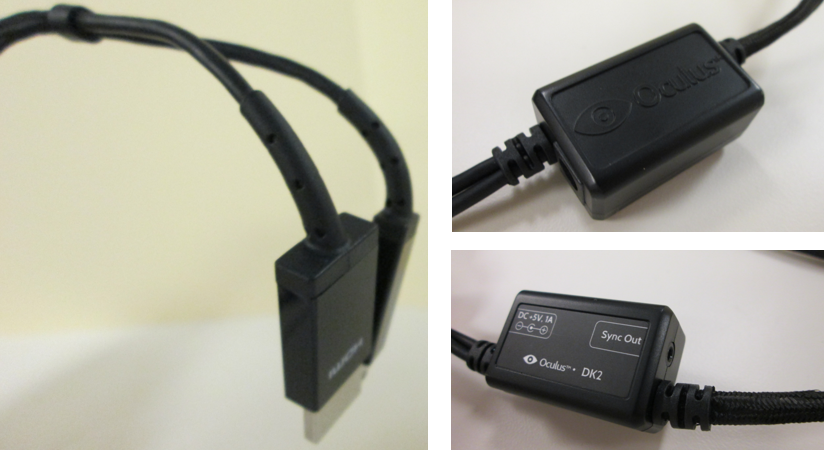
\includegraphics[width=0.9\textwidth]{Figures/DK2_Cable_Molded_Components.png}
  \caption{Rift DK 2 Cable molded components}
  \label{Cable_Molded_Components}
\end{figure}

\newpage

\section{Positional Tracking}
DK2 features positional tracking to a 2.5 meter distance at a 72 degree field of view. \\

Positional tracking is achieved using the Oculus SDK, based on data captured by the Positional Tracker sitting on the desk. The Positional Tracker captures snapshots of the LEDs modulating amplitudes in known patterns for LED identification, then sends the data back to the SDK for determination of position.

\subsection{Positional Tracker}
A 60hz Positional Tracker tracks the headset's spatial position within 2 meters with a 100 degree field of view using the LEDs on the front plate of the headset. This Positional Tracker is placed on the desk or atop a monitor in front of the headset with an unobstructed view of the LEDs. \\

See the Positional Tracker section of this document for more information on technical details of this system.

\subsection{LEDs}
DK2 includes 40 Vishay VSMY3850 850nm Infrared LEDs for positional tracking.  The LEDs are driven individually using constant current circuits that allow two brightness levels to be set.  The high or low setting is interfaced to the microcontroller via shift registers interfaced over SPI.  The LEDs and driving circuitry are placed on a flex PCB which is inserted into the front plastic assembly of the headset.

\subsection{Synchronization}
The IR LEDs are pulsed on only during the exposure period of the Positional Tracker.  This is achieved by driving synchronization pulse from the headset MCU to the Positional Tracker.  For DK2 the sync signal is connected to the Positional Tracker via a cable from the source (PC) side of the HMD interface.

\end{document}
